\section{Introduction}
\label{sec:intro}


\begin{figure}[t]
    \centering
    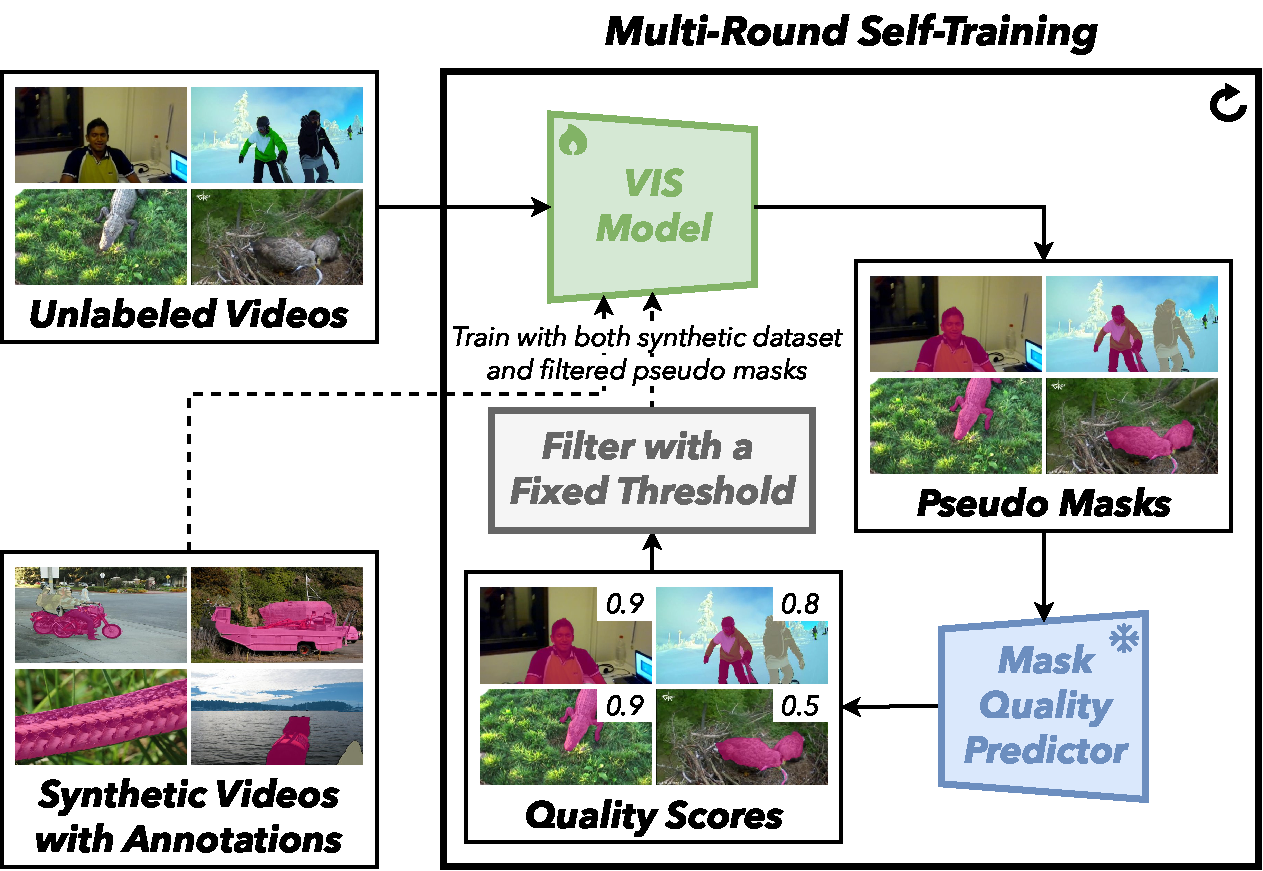
\includegraphics[width=1\linewidth]{figures/kaixuan_iccv_teaser.pdf}
    \caption{
        %The overall structure of AutoQ-VIS. The training dataset is initialized using the synthetic videos from VideoCutLER~\cite{videocutler}. In each round, we first train the VIS model on the established training dataset, then deploy it for pseudo-label generation on unlabeled video content. Following this, our quality predictor scores pseudo labels based on quality. Ultimately, we add the good-quality pseudo labels to the training dataset, which can be used for the next round of training. Through iterative training and dynamic dataset augmentation, we optimize the VIS model. The quality predictor is frozen during the self-training.
        %\textbf{Overview of the AutoQ-VIS pipeline.} We first initialize both the VIS model and the mask quality predictor by training on synthetic videos with annotations~\cite{videocutler} in the initial training stage. Then, in the multi-round self-training stage, at each round, the VIS model generates pseudo masks on unlabeled videos, which are then scored by the frozen quality predictor. Pseudo masks with high predicted quality scores are selected and added to the training set. The VIS model is retrained with both synthetic data and high-quality pseudo labels, enabling iterative self-training and progressive performance improvement.
        \textbf{AutoQ-VIS overview.} In the initial training stage, both the VIS model and the mask quality predictor are trained on synthetic videos with pseudo  annotations~\cite{videocutler}. During the multi-round self-training stage, the VIS model generates pseudo masks on unlabeled videos, which are then scored by the frozen quality predictor. Pseudo masks with high predicted quality are selected and added to the training set. The VIS model is subsequently retrained on both the synthetic data and the selected pseudo labels, enabling iterative refinement and progressive performance gains.
    }
    \label{fig:overall}
\end{figure}


Video Instance Segmentation (VIS) is the challenging task of simultaneously detecting, segmenting, and tracking object instances across video sequences~\cite{ytvis2019,wu2022seqformer,lin2020video,heo2022vita,wang2021end,zhang2023dvis}. This capability is fundamental for scene understanding in applications ranging from autonomous driving~\cite{driving_vis_dataset} to video content editing~\cite{vis_survey}. However, training high-performance VIS models typically requires pixel-level annotations across all frames~\cite{ytvis2019}. This process is expensive due to the labor-intensive nature of annotating temporal consistency and instance identities. As a result, there is an urgent need to develop unsupervised video instance segmentation frameworks that can accurately interpret video content and function effectively across diverse, unlabeled environments.
% To overcome this annotation bottleneck, we propose AutoQ-VIS, an unsupervised learning framework that eliminates manual labeling through iterative pseudo-label refinement with automatic quality assessment, enabling effective model training directly from unlabeled videos. \dimpp{this sentence does not fit here}
% ONUR: Follow this structure, separate paragraphs:
%1 Introduce the task with context and references.
%2 Highlight challenges and limitations of the state-of-the-art.
%3 Present your motivation: why this approach?
%4 Summarize the solution and its impact, with quantitative metrics

Prior work~\cite{motiongroup, emdriven, guessmove, bootstrapping, highly_probable_positive_features, transport_network, dense_video_seg} in unsupervised video segmentation predominantly addresses Video Object Segmentation (VOS), focusing on separating a single foreground object via motion or consistency cues. While OCLR~\cite{oclr} introduces unsupervised VIS that supports multiple instances, its predefined object count during training prevents dynamic adaptation to varying numbers of instances during inference. Furthermore, prior approaches~\cite{motiongroup, emdriven, guessmove, bootstrapping, oclr} rely on optical flow estimators (e.g.,  RAFT~\cite{raft}) that are trained on human-annotated datasets. VideoCutLER~\cite{videocutler} marks a breakthrough in unsupervised VIS and achieves unprecedented performance by demonstrating multi-instance segmentation without optical flow dependencies. Its core innovation lies in synthetic video generation via spatial augmentations of CutLER~\cite{cutler} pseudo-labels from ImageNet~\cite{imagenet}. However, VideoCutLER remains constrained by synthetic-to-real domain gaps and static instance modeling, i.e., the synthetic videos lack natural and realistic motion patterns. 
%\kaixuan{should we put mask scoring here? I can't find a smooth transition to put it here}
% ONUR: since we don't have a related work section, you can add more citations here

Building upon VideoCutLER's synthetic data paradigm, which generates training videos through spatial augmentations of static image pseudo-labels, we introduce AutoQ-VIS to address its critical domain gap limitation. While VideoCutLER's synthetic videos provide initial instance awareness, they lack natural motion patterns and real-world appearance variations, hindering adaptation to authentic video dynamics. Our framework bridges this synthetic-to-real domain gap through a self-training loop that progressively adds quality-filtered pseudo-labels from unlabeled real videos. Inspired by Mask Scoring R-CNN~\cite{maskscore}, which directly predicts mask quality scores via an auxiliary branch, we implement a quality assessment module for pseudo-label filtering of instance masks.
% As illustrated in~\cref{fig:overall}, our core innovation lies in integrating this mask quality prediction mechanism into video self-training---enhancing our model through progressive quality-assured pseudo labels augmentation.

% \begin{figure*}[t]
%     \centering
%     
\includegraphics[width=1\linewidth]{figures/overall.pdf}
%     \caption{
%         The overall structure of AutoQ-VIS. The training dataset is initialized using the synthetic videos from VideoCutLer~\cite{videocutler}. In each round, we first train the VIS model on the established training dataset, then deploy it for pseudo-label generation on unlabeled video content. Following this, our quality predictor scores pseudo labels based on quality. Ultimately, we add the good-quality pseudo labels to the training dataset, which can be used for the next round of training. Through iterative training and dynamic dataset augmentation, we optimize the VIS model. $^*$\textit{Frozen}: The quality predictor is frozen during the self-training.
%     }
%     \label{fig:overall}
% \end{figure*}

% The framework operates through three phases: \textbf{(1) Synthetic-to-Real Transition:} Initializing with VideoCutLER's synthetic data to bootstrap fundamental instance awareness (\cref{sec:initial_model}). \textbf{(2) Automatic Pseudo Label Quality Assessment:} Selecting reliable pseudo-labels via a pre-trained frozen quality predictor (\cref{sec:multi_round_training}). \textbf{(3) Dynamic Data Augmentation:}  Gradually expanding the training dataset with confidence-filtered real video annotations (\cref{sec:multi_round_training}).

%As shown in \cref{fig:overall}, our framework, 
AutoQ-VIS advances unsupervised video instance segmentation through an iterative self-training paradigm with quality-aware pseudo-label selection (\cref{fig:overall}). The system initializes using synthetic video data from VideoCutLER, which provides pseudo-labels to bootstrap a VideoMask2Former~\cite{mask2former, videomask2former} VIS model and a specialized mask quality predictor (\cref{sec:initial_model}). The mask quality predictor 
%employs a Mask Scoring R-CNN-inspired architecture to 
estimates mask IoU quality scores by analyzing frame-level features and mask predictions. During multi-round optimization, the VIS model generates pseudo-labels on unlabeled videos, which are then scored by the quality predictor. High-quality pseudo-labels surpassing a fixed threshold are progressively incorporated into the training set, enabling dataset augmentation without any human supervision (\cref{sec:multi_round_training}). To enhance the mask head training, we employ a DropLoss that zeros out mask losses whose maximum ground‑truth overlap falls below 0.01 (\cref{sec:droploss}).  By alternating rounds of VIS training (with occasional weight resets) and quality‑based dataset expansion, AutoQ‑VIS dynamically enriches its training dataset and steadily sharpens segmentation performance. 

% \todo{mention uvo results}
AutoQ-VIS establishes a new state-of-the-art in unsupervised video instance segmentation, achieving 52.6\% $\text{AP}_{50}$ on the YouTubeVIS-2019 validation set~\cite{ytvis2019}. This represents a significant +4.4\% $\text{AP}_{50}$ improvement over the previous best-performing method VideoCutLER~\cite{videocutler}, demonstrating our framework's effectiveness in motion pattern understanding and instance-level discrimination. To further validate the approach's generalizability, we conduct additional evaluation on the UVO-Dense benchmark~\cite{uvo}, where our method achieves consistent performance gains (1.1\% $\text{AP}_{50}$ improvement over the previous state-of-the-art approaches) under dense object scenarios.

Our key contributions are threefold: \textbf{(1) Annotation-Free VIS Framework:} We propose AutoQ-VIS, an unsupervised framework that overcomes annotation dependency through cyclic pseudo-label refinement with automated quality control, enabling video instance segmentation training directly from unlabeled videos. \textbf{(2) Automatic Quality Assessment:} We propose a simple quality predictor that reliably filters pseudo labels across self-training rounds. \textbf{(3) New State-of-the-art Performance:} Our AutoQ-VIS achieves 52.6 ${\text{AP}_{50}}$ on YouTubeVIS-2019~\cite{ytvis2019} \texttt{val} split, surpassing the previous state-of-the-art VideoCutLER~\cite{videocutler} by 4.4 ${\text{AP}_{50}}$.